% this file is called up by thesis.tex
% content in this file will be fed into the main document

%: ----------------------- name of chapter  -------------------------
\chapter{Analiza wymagań} % top level followed by section, subsection


%: ----------------------- paths to graphics ------------------------

% change according to folder and file names
\ifpdf
    \graphicspath{{3/figures/PNG/}{3/figures/PDF/}{3/figures/}}
\else
    \graphicspath{{3/figures/EPS/}{3/figures/}}
\fi

%: ----------------------- contents from here ------------------------

Tem rodział opisuje wymagania które powinny być spełniane przez poszczególne, przykładowe aplikacje korzystające z serwisu UniversalSynthesizer. Podstawową funkcją serwisu jest udostępnianie usługi zamiany tekstu na mowę. Zaletą niniejszego systemu jest jego otwartość, możliwość wykorzystania innych niż proponowane syntezatorów mowy, łatwy dostęp przez web service, stosunkowo prosty sposób rozbudowy oraz możliwość jego wykorzystania do różnych celów na różnych platformach. Cechy te należy zademonstrować na przykładzie kilku prostych aplikacji, które muszą spełniać pewne jasno określone wymagania funkcjonalne i niefunkcjonalne opisane poniżej. 
\section{Wymagania funkcjonalne}

\subsection{Automatyczne dyktando}
Jest to prosta aplikacja dostępna dla użytkowników w formacie strony internetowej. Jej głównym celem jest wykorzystanie funkcji UniversalSynthesizer do dyktowania treści którą użytkownik zapisuje. Po odczytaniu całego tekstu i wysłaniu przez użytkownika formularza, jest on porównywany z tekstem oryginalnym w ten sposób może ćwiczyć swoją ortografie. Dużą zaletą jest to, że aplikacja ta nie jest ograniczona do jednego języka oraz fakt, że użytkownik sam podaje tekst.
\subsubsection {Przypadki użycia} 
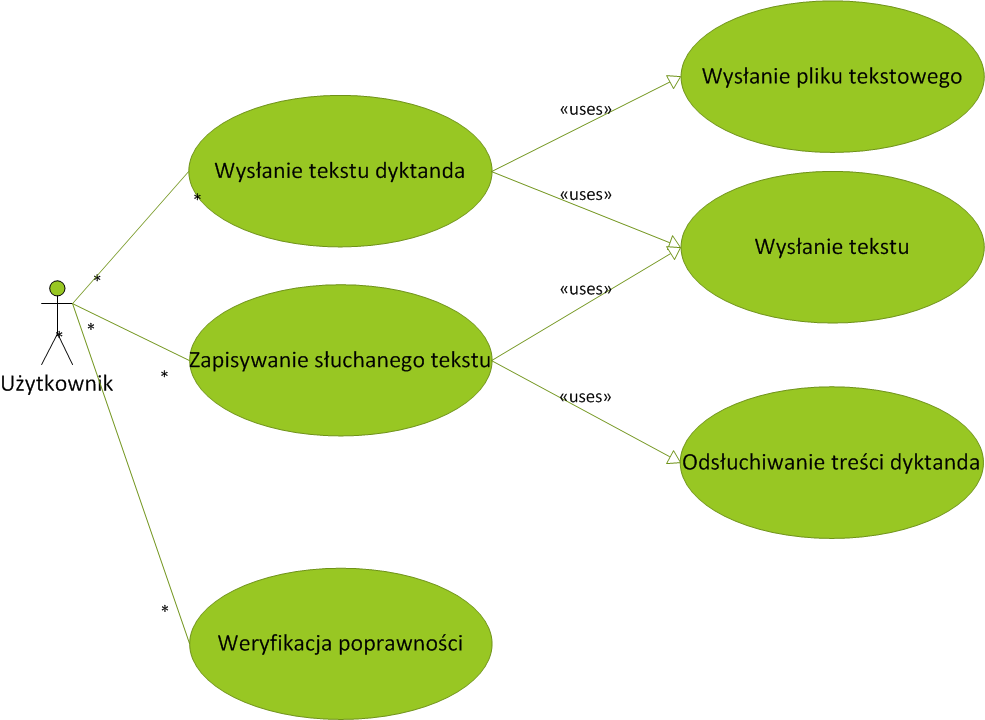
\includegraphics[scale=0.55]{useCaseDictando.png} 
\subsubsection{Wymagania funkcjonalne}
\begin{enumerate}
	\item Obsługiwanie więcej niż jednego języka
		\begin{enumerate}
			\item polski
			\item angielski
			\item francuski
		\end{enumerate}
	\item Możliwość podania tekstu źródłowego
		\begin{enumerate}
			\item w formie tekstu wpisywanego na stronie
			\item jako plik tekstowy, wysyłany na serwer
		\end{enumerate}
	\item Umożliwienie użytkownikowi odsłuchania wysłanego tekstu w wybranym przez niego języku
	\item Umożliwienie użytkownikowi wprowadzania tekstu jednocześnie z odsłuchiwaniem
	\item Wygenerowanie i wyświetlenie raportu o ilości błędów popełnionych przez użytkownika
\end{enumerate}
\subsection{Lektor RSS}
Jest to aplikacja webowa, które głównym celem jest odczytywanie użytkownikowi wiadomości RSS pobieranych z podanych przez niego źródeł. Należy zwrócić uwagę na duża zaletę tej aplikacji jaką jest fakt, że w zależności od języka wiadomości RSS jest ona odczytywana przez lektora odpowiedzialnego za ten język, oczywiście przy założeniu, że UniversalSynthesizer obłusguje język wiadomości.
\subsubsection{Przypadki użycia}
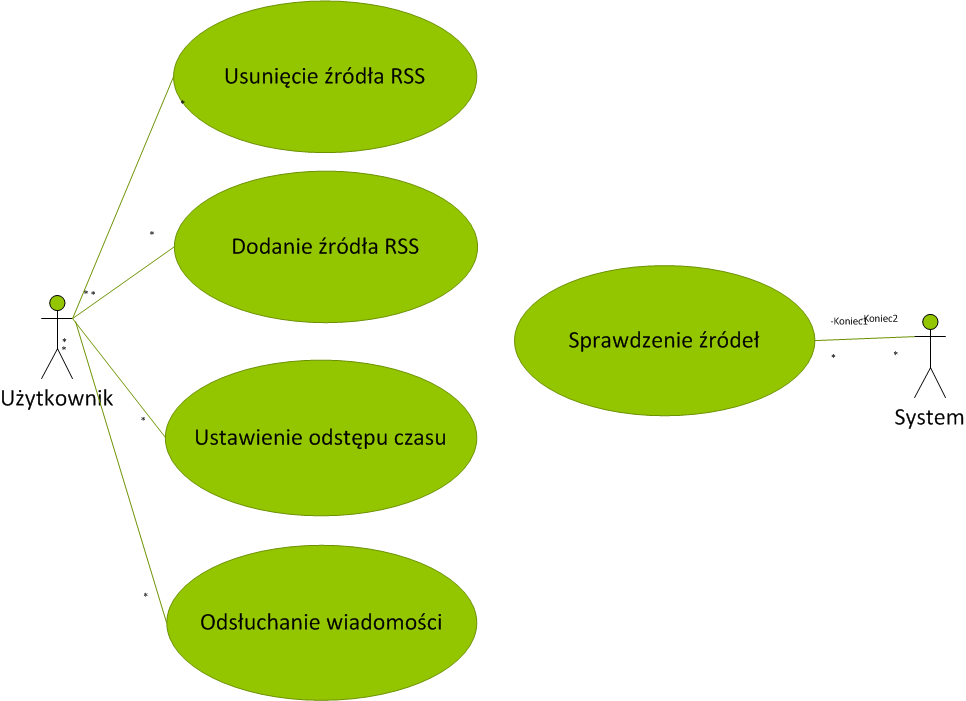
\includegraphics[scale=0.55]{useCaseRSS.png} 
\subsubsection{Wymagania funkcjonalne}
\begin{enumerate}
	\item Możliwość dodania źródła RSS
	\item Możliwość usunięcia źródła RSS
	\item Obsługiwanie więcej niż jednego języka wiadomości
		\begin{enumerate}
			\item polski
			\item angielski
			\item francuski
		\end{enumerate}
	\item Automatyczne sprawdzanie czy któreś ze źródeł nie zawiera nowej wiadomości
	\item Możliwość ustawienia odstępów czasowych pomędzy sprawdzaniem przez system źródeł
	\item Automatyczne Odczytanie użytkownikowi nowych wiadomości (w przypadku istnienia) 
\end{enumerate}  


% ---------------------------------------------------------------------------
%: ----------------------- end of thesis sub-document ------------------------
% ---------------------------------------------------------------------------

